\documentclass[12pt, a4paper]{scrartcl}


\usepackage{lmodern} 		% Diese beiden packages sorgen für echte
\usepackage[T1]{fontenc}	% Umlaute.
\usepackage[utf8]{inputenc}
\usepackage[ngerman]{babel}

\usepackage[pdfpagelabels,pdfstartview = FitH,bookmarksopen = true,bookmarksnumbered = true,linkcolor = black,plainpages = false,hypertexnames = false,citecolor = black, breaklinks]{hyperref}
\usepackage{url}



%Spezialpakete Zeichnen
\usepackage{tikz}
\usepackage{fp}
\usepackage{xcolor}
% TikZ-Bibliotheken
\usetikzlibrary{arrows}
\usetikzlibrary{shapes}
\usetikzlibrary{decorations.pathmorphing}
\usetikzlibrary{decorations.pathreplacing}
\usetikzlibrary{decorations.shapes}
\usetikzlibrary{decorations.text}
\usetikzlibrary{patterns}

\usepackage{pgfplots}
%%FIGUR
%\begin{figure}[htbp]
%\centering
%\includegraphics[width=15cm]{Bild1}%
%\caption{Experimental set-up}%
%\label{1}
%\end{figure}

%%BILD MIT PICINS NEBEN TEXT SETZEN
%\piccaption{Caption\label{label}}
%\parpic[r]{\fbox{\includegraphics [width=5cm, keepaspectratio]{bild.png}}}
%


%% ZWEI BILDER NEBENEINANDER.
%% Schau, dass die minipages insgesamt nie mehr als 1.0\textwidth haben.
%% Um ein drittes oder viertes Bild einzufügen, ergänze einfach um weitere minipages.
% \begin{figure}[!htb]
% \centering
%   \minipage{0.3\textwidth}
%     \fbox{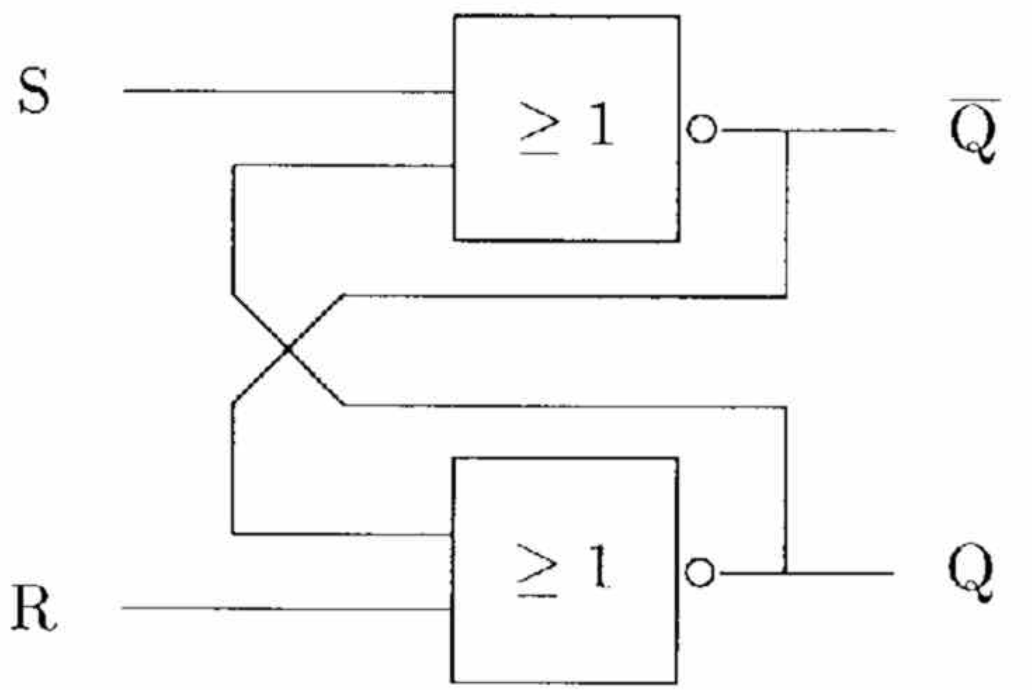
\includegraphics[height=2.5cm, keepaspectratio]{rsflipflop.png}}%
%     \caption{RS-Flipflop}%
%     \label{fig:rsflipflop}
%   \endminipage\hspace{1cm}
% %
%   \minipage{0.4\textwidth}
%     \fbox{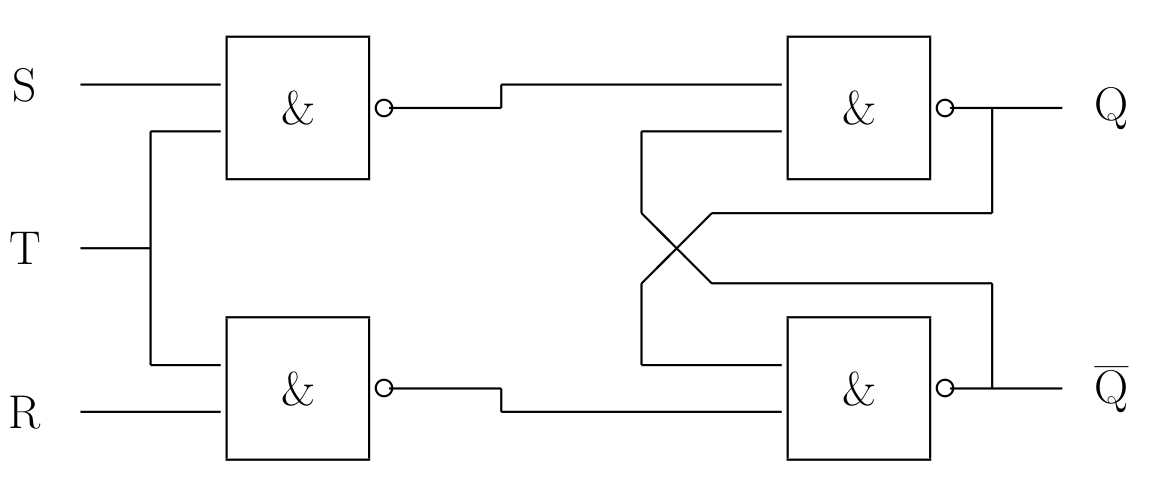
\includegraphics[height=2.5cm, keepaspectratio]{rsflipfloptakt.png}}%
%     \caption{getaktetes RS-Flipflop}%
%     \label{fig:rsflipfloptakt}
%   \endminipage
% \end{figure}




%------------------------------------------


\begin{document}

\section*{Drawing in \LaTeX}
\tableofcontents
\pagebreak

\subsection{Notizen}

\begin{verbatim}
% Spezialpakete
\usepackage{tikz}
\usepackage{fp}
\usepackage{tikz}
\usepackage{xcolor}
% TikZ-Bibliotheken
\usetikzlibrary{arrows}
\usetikzlibrary{shapes}
\usetikzlibrary{decorations.pathmorphing}
\usetikzlibrary{decorations.pathreplacing}
\usetikzlibrary{decorations.shapes}
\usetikzlibrary{decorations.text}

Command:
\tikz[options]{tikz commands}
\end{verbatim}

oder

\begin{verbatim}
   \begin{tikzpicture}
      blabla
   \end{tikzpicture}

\end{verbatim}


\begin{itemize}
   \item Innerhalb der tikzpicture-Umgebung keine leeren Zeilen!

   \item Wenn keine Grösse angegeben, werden die Werte in Klammern als $cm$ interpretiert.

   \item Das Koordinatensystem beginnt in der unteren linken Ecke der Arbeitsfläche.

   \item Benutze nicht Einheiten, sondern skaliere das Gesamtbild. Und falls nötig, zeige den Rechteck der Arbeitsfläche an.
   \begin{verbatim}
   \usetikzlibrary{backgrounds}
   \begin{tikzpicture}[scale=.8, show background rectangle]
   \end{verbatim}

   \item Falls Text in Nodes vorhanden ist: benutze
   \begin{verbatim}
    \begin{tikzpicture}[scale=.9, transform shape]
    \end{verbatim} Transform shape: Damit Node-Text mitskaliert wird.

\end{itemize}

\subsection{Links}
\begin{itemize}
   \item \url{http://www.math.uni-leipzig.de/~hellmund/LaTeX/pgf-tut.pdf}
   \item \url{http://www.math.tugraz.at/~huss/new/teaching/computermathematik09/dateien/tikz_demonstration.pdf}
   \url{http://www.texample.net/tikz/}
   \item \url{https://www.sharelatex.com/blog/2013/08/27/tikz-series-pt1.html}
\end{itemize}




\pagebreak
\section{Basics}
\subsection{Gerade Linien zeichnen, relative Koordinaten}
\begin{tikzpicture}
\draw (0,0) -- (2, 2);
\end{tikzpicture}
%
\hspace{1cm}
%
\begin{tikzpicture}
   \draw (0,0) -- +(6.2, 0.7);
\end{tikzpicture}



\subsection{Pfeile}
\begin{tikzpicture}
\draw[->] (0,0) -- (2, 2);
% mit "+" werden relative Koordinaten angegeben
\draw[<->>, line width=3pt] (2,0) -- +(2, 2);
\draw[->, line width=2pt] (4,0) -- +(1, 1.5);
\draw[<-, red, dashed, line width = 2pt] (6,2) -- (8,0);
\draw[->, blue, dotted, line width = 2pt] (8,0) -- (10,3);
\end{tikzpicture}

{\renewcommand{\arraystretch}{2}%
\begin{tabular}{l l }
\begin{tikzpicture}
\draw[->] (0,0) -- (2,0);
\end{tikzpicture} & $\backslash draw[->]$ \\

\begin{tikzpicture}
\draw[dotted, >->>](0,0) -- (2,0);
\end{tikzpicture} & $\backslash draw[dotted, >->>]$\\

\begin{tikzpicture}
\draw[|<->|] (0,0) -- (2,0);
\end{tikzpicture} & $\backslash draw[|<->|]$\\

\begin{tikzpicture}
\draw[loosely dashed] (0,0) -- (2,0);
\end{tikzpicture} & $\backslash draw[loosely\ dashed]$\\

\begin{tikzpicture}
\draw[densely dotted] (0,0) -- (2,0);
\end{tikzpicture} & $\backslash draw[densely \ dotted]$ \\

\begin{tikzpicture}
\draw[->] (0,0) .. controls (.4,-.4) .. (2, 0);
\end{tikzpicture} & $\backslash draw[->] (0,0) .. controls (.4,-.4) .. (2, 0)$
\end{tabular}


\subsection{Polarkoordinaten; Geschlossene Figur}

\begin{verbatim}
   Polarkoordinaten: (winkel:radius). Winkel auch negativ möglich
   Zum Anfangspunkt verbinden: -- cycle;
\end{verbatim}
\begin{tikzpicture}
\draw (0:1cm) -- (72:1cm) -- (2*72:1cm) --
(3*72:1cm) -- (4*72:1cm) -- cycle;
\end{tikzpicture}
%
\hspace{2cm}
%
\begin{tikzpicture}
   \draw[blue, line width = 2pt] (0:1.5cm) -- (60:1.5cm) -- (2*60:1.5cm) -- (3*60:1.5cm) -- (4*60:1.5cm) --(-60:1.5cm) -- cycle;
\end{tikzpicture}
%
\hspace{2cm}
%
\begin{tikzpicture}
\draw[color=red] (0,0) -- (40:1);
\draw[color=blue] (0,0) -- (160:1);
\draw[thick] (0,0) -- (90:1);

\end{tikzpicture}


\subsection{Einfache Figuren}
\begin{tikzpicture}
   \draw (0, 0) rectangle (2, 1);
   \draw[color=red] (4, 0) circle (.5);
   \draw (6, 0) ellipse (.7 and 0.5);
\end{tikzpicture}






\section{Komplexeres}

\subsection{Fills}

\begin{tikzpicture}
\fill (0,0) circle (0.25);
\fill[red] (1,0) circle (0.25);
\fill[blue] (2,0) circle (0.25);
\shade[ball color=green] (3,0) circle (0.25);
\fill[orange] (4,0) circle (0.25);
\fill[green,opacity=0.5] (4.25,0) circle (0.25);
\end{tikzpicture}

\subsection{Clipping und Scope}
After a clip command, all subsequent drawings are clipped, only the parts inside the clipping region are drawn.

Use the scope environment to restrict the effect of clipping.

\begin{tikzpicture}
\draw (-2, 1.5) rectangle (2, -1.5);
\begin{scope}
\clip (-0.5, 0) circle (1); % Über clips wird eine abgeschlossene Fläche definiert. Sobald diese gemacht ist, wird nur noch das gezeichnet, was innerhalb dieser Fläche liegt, sonst nichts.
\clip ( 0.5, 0) circle (1);
\fill[color=gray!40] (-2,1.5)
rectangle (2,-1.5);
\end{scope} % Scope begrenzt die Wirkung des clippings. Alles ausserhalb von scope wird wieder gezeichnet.
\draw (-0.5, 0) circle (1);
\draw ( 0.5, 0) circle (1);
\end{tikzpicture}

\subsection{Kurvenlinien}
\begin{tikzpicture}
  \draw[line width = 2pt] (0,0) .. controls (2,1) and (4,-2) .. (8,0);
  \draw[dotted] (0,0)--(8,0);
\end{tikzpicture}

\begin{tikzpicture}
% Direkte eingabe der Kontrollpunkte:
\draw (0,0) .. controls (0,1) and (1,1) .. (2, 2);
% Die Line krümmt sich um 30 Grad nach Links:
\draw[bend left=30] (3,0) to (4, 2);
% aus- und eingehenden Winkel festlegen:
\draw (6,0)  to [out=90, in=-90] (7, 2) to [out = 20, in = -90] (10, 1);
\end{tikzpicture}

\subsection{Nodes}

\begin{verbatim}
\node[Options] (node name) at (x,y) {TeX content of node}
\end{verbatim}

\begin{tikzpicture}[scale=.9, transform shape] %Transform shape: Damit Nodes mitskaliert werden.
\tikzstyle{every node} = [circle, fill=gray!30]
\node (a) at (0, 0) {A};
\node (b) at +(0: 1.5) {B};
\node (c) at +(60: 1.5) {C};
\foreach \from/\to in {a/b, b/c, c/a}
\draw [->] (\from) -- (\to);
\end{tikzpicture}

\begin{tikzpicture}
\node (A) at (0,0) [circle,shade,draw] {$\sin(x)$};
\node (B) at (3,0) {$\cos(x)$};
\node (C) at (6,0) [fill=red!50] {$-\sin(x)$};
\draw[->, blue!50, very thick] (A) to[bend right=20]
node[above] {$\frac{\partial}{\partial x}$} (B);
\draw[->, blue!50, very thick] (B) to (C);
\draw[<->, thick] (A) to[out=45, in=135] (C);
\end{tikzpicture}



\section{Varia}
\subsection{grid}
\begin{tikzpicture}
\draw[step=1cm,gray,very thin] (-1,-1) grid (2,2);
\end{tikzpicture}
%
\begin{tikzpicture}
\draw[step=0.5cm,gray,very thin] (-1.5,-1.5) grid (1.5,1.5);
\end{tikzpicture}
%
\begin{tikzpicture}
\draw[step=1mm,gray,very thin] (-1.5,-1.5) grid (1.5,1.5);
\end{tikzpicture}

\subsection{Axes}
\begin{tikzpicture}
\draw[step=1cm,gray!20,very thin] (-1.9,-1.9) grid (5.9,5.9);
\draw[thick,->] (0,0) -- (4.5,0) node[anchor=north west] {x axis};
\draw[thick,->] (0,0) -- (0,4.5) node[anchor=south east] {y axis};
\foreach \x in {0,1,2,3,4}
\draw (\x cm,1pt) -- (\x cm,-1pt) node[anchor=north] {$\x$};
\foreach \y in {0,1,2,3,4}
\draw (1pt,\y cm) -- (-1pt,\y cm) node[anchor=east] {$\y$};
\end{tikzpicture}

%
\subsection{Color fillings}
\begin{tikzpicture}
\filldraw[fill=blue!40!white, draw=black] (0,0) rectangle (2,2);
\end{tikzpicture}
%
%
\begin{tikzpicture}
\shade[left color=blue,right color=red] (0,0) rectangle (2,2);
\end{tikzpicture}
%
\begin{tikzpicture}
\shade[top color=blue,bottom color=red] (0,0) rectangle (2,2);
\end{tikzpicture}
%
\begin{tikzpicture}
\shadedraw[inner color=blue,outer color=red, draw=black] (0,0) rectangle (2,2);
\end{tikzpicture}


\vfill
\newpage
\section{Plots}
Braucht \verb|\usepackage{pgfplots}|


\fbox{
\begin{tikzpicture}[xscale=1,yscale=0.8,samples=400]
	\begin{axis}[
	axis x line=bottom,axis y line=left,
	xlabel = $x$,
	ylabel = {$y$},
	legend pos=north west,
	]

	%red line
	\addplot [
	domain=-10:10,
	samples=400,
	color=red,
	]
	{-2*x^2 +3*x + 100};
		\addlegendentry{$f(x)$}

	%Blue line
	\addplot [
	domain=-10:10,
	samples=400,
	color=blue,
	]
	{100*exp( (-x^2)/10)*sin(270*x)};
		\addlegendentry{$g(x)$}
	\end{axis};
\end{tikzpicture}
}

\fbox{
\begin{tikzpicture}[xscale=1,yscale=0.8,samples=400]
	\begin{axis}[
	ticks=none,
	ymin=-1,
	ymax=5,
	xmin=-3,
	xmax=5.2,
	axis x line=bottom,axis y line=left,
	xlabel = {$x$},
	ylabel = {$y$},
	legend pos=north east,			% legend location
	every axis x label/.style={		% set nice axis labels
		at={(ticklabel* cs:1.05)},
		anchor=west,
	},
	every axis y label/.style={
		at={(ticklabel* cs:1.05)},
		anchor=south,
	},
	]

	%red line
	\addplot [
	domain=1:5,
	samples=400,
	color=red,
	]
	{1/x*cos(360*x)};
	\addlegendentry{$1/x*cos(360*x)$}

	%blue line
	\addplot [
	domain=-4:1,
	samples=400,
	color=blue,
	]
	{exp(-(x-1)};
	\addlegendentry{$exp(-(x-1))$}
	\end{axis};
\end{tikzpicture}
}










\vfill
\newpage
\section{Meine Zeichnungen}
\subsection{Praktikumsbericht Kern- und Teilchenphysik: Positronenvernichtung}
\subsubsection{1}
\fbox{
	\begin{tikzpicture}[scale=0.6, every node/.style={scale=0.8}]
		%
		%22Na
		\draw[line width = 3pt] (0,10) -- node[above=1mm]{\Large{$^{22}$\textbf{Na}}} (4,10) node[right=1mm]{$\tau_{1/2} = 2.6$a};
		%
		%Ne angeregter Zustand
		\draw[line width = 3pt] (5,5) -- node[above]{$\tau_{1/2} = 3$ps} (9,5);
		%
		%Ne Grundzustand
		\draw[line width = 3pt] (5,0) -- node[below=1mm]{\Large{$^{22}$\textbf{Ne}}} (9,0);
		%
		%Photon
		\draw[line width = 1.5pt, decorate, decoration=snake] (7,4.9)-- node[right=1mm]{$E_\gamma = 1.275$ MeV} (7,0.2);
		\draw[->, line width = 1.5pt] (7,0.2)--(7,0.1);
		%
		%beta+ 90%
		\draw[->, line width = 1.5pt] (3,10) -- node[right=1mm]{$\beta^{+}$, 90$\%$} (4.9,5.1);
		%
		%beta+ 0.5%
		\draw[->, line width = 1.5pt, style = dashed] (3,10) -- node[left=1mm]{$\beta^{+}$, 0.05$\%$} (4.9,0.1);
	\end{tikzpicture}
}

\subsubsection{2}

\fbox{ % Second picture
	\begin{tikzpicture}[scale=0.5, every node/.style={scale=0.8}]
		%100MHz
		\draw[line width = 1.5pt] (0,11) -- +(0.5, 0)-- +(0.5, 0.5) -- + (1, 0.5) -- +(1, 0)--
		+(1.5, 0)-- +(1.5, 0.5) -- + (2, 0.5) -- +(2, 0)-- node[above=5mm]{100MHz}
		+(2.5, 0)-- +(2.5, 0.5) -- + (3, 0.5) -- +(3, 0)--
		+(3.5, 0)-- +(3.5, 0.5) -- + (4, 0.5) -- +(4, 0)--
		+(4.5, 0)-- +(4.5, 0.5) -- + (5, 0.5) -- +(5, 0)
		;
		%
		%1kHz
		\draw[line width = 1.5pt] (6.5,11) -- +(0.5, 0)-- +(0.5, 0.5) -- + (1, 0.5) -- +(1, 0)-- node[above=5mm]{1kHz}
		+(4.5, 0)-- +(4.5, 0.5) -- + (5, 0.5) -- +(5, 0)-- +(5.5,0);
		%
		%Pfeil 100MHz
		\draw[->, line width = 1.5pt] (2.5, 10.5) -- (2.5, 9.1);
		%
		%Pfeil 10kHz
		\draw[->, line width = 1.5pt] (9, 10.5) -- (9, 9.1);
		%
		%Prescaler
		\draw[] (1.1,8) rectangle +(2.8,1);
		\node[] at (2.5, 8.5) {Prescaler};
		%
		%Diskriminator
		\draw[] (6.9,8) rectangle +(4.2,1);
		\node[] at (9, 8.5) {Diskriminator};
		%
		%TAC
		\draw[] (4.825,4.5) rectangle +(1.8,1);
		\node[] at (5.75, 5) {TAC};
		%
		%ADC
		\draw[] (4.825,1.5) rectangle +(1.8,1);
		\node[] at (5.75, 2) {ADC};
		%
		%Rechner
		\draw[] (8.4,1.5) rectangle +(2.6,1);
		\node[] at (9.75, 2) {Rechner};
		%
		%Pfeil Diskriminator- TAC
		\draw[->, line width = 1.5pt] (9, 7.9) -- node[right=1mm]{Start} (6.6, 5.6);
		%
		%Pfeil Prescaler-TAC
		\draw[->, line width = 1.5pt] (2.5, 7.9) -- node[left=1mm]{Stopp} (4.8, 5.6);
		%
		%Pfeil TAC-ADC
		\draw[->, line width = 1.5pt] (5.75, 4.4) -- (5.75, 2.6);
		%
		%Pfeil ADC-Rechner
		\draw[->, line width = 1.5pt] (6.8, 2) -- (8.2, 2);
	\end{tikzpicture}
}


\subsubsection{3}


\begin{tikzpicture}
	 \node at (2,0) [draw,thick,minimum width=2cm,minimum height=1cm] {BaF$_2$-Detektor};
	 %
	 \node at (7.2,1.2) [draw,thick,minimum width=2cm,minimum height=1cm] {Verstärker};
	 %
	 \node at (7.2,-1.2) [draw,thick,minimum width=2.2cm,minimum height=1cm, text width = 2.2cm] {\small{Pulse Height Analyser}};
	 %
	 \node at (11,1.2) [draw,thick,minimum width=2cm,minimum height=1cm]{Delay};
	 %
	 \node at (11,-1.2) [draw,thick,minimum width=2cm,minimum height=1cm, text width = 2.4cm] {\small{Einkanal- diskriminator}};
	 %
	 \node at (14,0) [draw,thick,minimum width=2cm,minimum height=1cm] {ADC};
	 %
	 \node at (2,-2) [thick,minimum width=2cm,minimum height=1cm] {Hochspannung};
	 %
	 %Hochspannung
	 \draw[->, line width = 1.5pt, style=dashed] (2, -1.7) -- (2, -0.7);
	 %
	 %Detektor-Verstärker
	 \draw[->, line width = 1.5pt] (3.7,0) -- (4.5,0)--(4.5, 1.2)--(6, 1.2);
	 %
	 %Detektor-PHA
	 \draw[->, line width = 1.5pt] (4.5,0) -- (4.5, -1.2) -- (5.8, -1.2);
	 %
	 %Verstärker-Delay
	 \draw[->, line width = 1.5pt] (8.5, 1.2)--(9.8,1.2);
	 %
	 %PHA-EKDisrk
	 \draw[->, line width = 1.5pt] (8.6, -1.2)--(9.5,-1.2);
	 %
	 %Delay-ADC
	 \draw[->, line width = 1.5pt] (12.1, 1.2)--(14,1.2)--node[right=1mm]{Signal} (14, 0.6);
	 %
	 %EKDiskr - ADC
	 \draw[->, line width = 1.5pt] (12.4, -1.2)--(14,-1.2)--node[right=1mm]{Gate} (14, -0.6);
\end{tikzpicture}


\subsubsection{4}

\fbox{
   	\begin{tikzpicture}[scale=0.55, every node/.style={scale=0.55}]
	   	%QUELLE
	   	\draw[line width=1.5pt] (0, 0) circle (0.5) node [above = 4mm] {$^{22}Na$-Quelle};
	   	\fill[fill=gray]
	   	(0, 0) circle (0.3);
	   	%
	   	%Hintergrund RECHTS
	   	\fill[fill=blue!40] (1.5,0.5)--(4.5,-0.5)--(1.5,-0.5)--cycle;
	   	\fill[fill=green!40] (1.5,0.5)--(4.5,0.5)--(4.5,-0.5)--cycle;
	   	%
	   	%Hintergrung LINKS
	   	\fill[fill=blue!40] (-1.5,-0.5)--(-1.5,0.5)--(-4.5,-0.5)--cycle;
	   	\fill[fill=green!40] (-4.5,-0.5)--(-4.5,0.5)--(-1.5,0.5)--cycle;
	   	%
	   	%Hochspannugn
	   	\node at (0,2) [thick,minimum width=2cm,minimum height=1cm, ]{Hochspannung};
	   	%
	   	%Koinzidenzeinheit
	   	\node at (0,-6.6) [draw, thick,minimum width=3.5cm,minimum height=1cm, fill=blue!40]{Koinzidenzeinheit};
	   	%
	   	%ADC
	   	\node at (0,-8.9) [draw, thick,minimum width=3.5cm,minimum height=1cm]{ADC};
	   	%
	   	%Rechner
	   	\node at (5,-8.9) [draw, thick,minimum width=3cm,minimum height=1cm]{Rechner};
	   	%
	   	%Pfeil Koinzidenzeinheit - ADC
	   	\draw[->, line width=1.5pt] (0, -7.2) -- node[right = 1mm]{Gate}(0, -8.3);
	   	%
	   	%Pfeil ADC-Rechner
	   	\draw[->, line width=1.5pt] (1.8, -8.9) -- (3.4, -8.9);
	   	%
	   	%TAC
	   	\node at (-3.5,-11.2) [draw, thick,minimum width=3cm,minimum height=1cm, fill=green!40]{TAC};
	   	%
	   	%Pfeil TAC-ADC
	   	\draw[->, line width=1.5pt] (-3.5, -10.6) -- (-3.5, -8.9)-- node[above=1mm]{Signal} (-1.8, -8.9);

	   	%%%%%%%%%%%%%%%%%%%%%%%%%%%%%%%%%%%%%%
	   	%RECHTE SEITE
	   	%Detektor
	   	\node at (3,0) [draw,thick, text width = 2.7cm, minimum height=1cm,] {BaF$_2$-Detektor};
	   	\draw[fill=gray] (1.2, -0.35) rectangle (1.5, 0.35);
	   	%
	   	%Hochspannung Pfeil
	   	\draw[->, line width=1.5pt, style = dashed] (1.5,2) -- (3,2)-- (3, 0.6);
	   	%
	   	%Verstärker
	   	\node at (3, -2.4)  [draw,thick,minimum width=2.2cm,minimum height=1cm, text width = 2.7cm, align=center, fill=blue!40] {Verstärker, PHA};
	   	%
	   	%Pfeil Detektor-PHA
	   	\draw[->, line width=1.5pt] (3,-0.6) -- (3,-1.8);
	   	%
	   	%EKDiskr
	   	\node at (3, -4.8)  [draw,thick,minimum width=2.2cm,minimum height=1cm, text width = 2.7cm, align=center, fill=blue!40] {Einkanal-diskriminator};
	   	%
	   	%Pfeil PHA - EKDiskr
	   	\draw[->, line width=1.5pt] (3,-3) -- (3,-4.2);
	   	%
	   	%Pfeil EKDiskr-Koinzidenzeinheit
	   	\draw[->, line width=1.5pt] (3,-5.4) -- (3,-6.6) -- (1.8, -6.6);
	   	%
	   	% CDF
	   	\node at (7.5,0) [draw,thick, text width = 3cm, minimum height=1cm, fill=green!40, align=center] {Constant Fraction Diskriminator};
	   	%
	   	%Pfeil Detektor-CDF
	   	\draw[->, line width=1.5pt] (4.6,0) -- (5.8,0);
	   	%
	   	%Delay
	   	\node at (7.5, -2.4)  [draw,thick,minimum width=2.2cm,minimum height=1cm, text width = 2.7cm, align=center, fill=green!40] {Delay};
	   	%
	   	%Pfeil CDF-Delay
	   	\draw[->, line width=1.5pt] (7.5,-0.9) -- (7.5,-1.8);
	   	%
	   	%Pfeil Delay-TAC
	   	\draw[->, line width=1.5pt] (7.5,-3) -- (7.5,-11.2)-- node [above = 1mm]{Stopp} (-1.9, -11.2);
	   	%%%%%%%%%%%%%%%%%%%%%%%%%%%%%%%%%%%%%%
	   	%%%%%%%%%%%%%%%%%%%%%%%%%%%%%%%%%%%%%%
	   	%%%%%%%%%%%%%%%%%%%%%%%%%%%%%%%%%%%%%%
	   	%LINKE SEITE
	   	%Detektor
	   	\node at (-3,0) [draw,thick, text width = 2.7cm, minimum height=1cm,] {BaF$_2$-Detektor};
	   	\draw[fill=gray] (-1.2, -0.35) rectangle (-1.5, 0.35);
	   	%
	   	%Hochspannung Pfeil
	   	\draw[->, line width=1.5pt, style = dashed] (-1.5,2) -- (-3,2)-- (-3, 0.6);
	   	%
	   	%Verstärker
	   	\node at (-3, -2.4)  [draw,thick,minimum width=2.2cm,minimum height=1cm, text width = 2.7cm, align=center, fill=blue!40] {Verstärker, PHA};
	   	%
	   	%Pfeil Detektor-PHA
	   	\draw[->, line width=1.5pt] (-3,-0.6) -- (-3,-1.8);
	   	%
	   	%EKDiskr
	   	\node at (-3, -4.8)  [draw,thick,minimum width=2.2cm,minimum height=1cm, text width = 2.7cm, align=center, fill=blue!40] {Einkanal-diskriminator};
	   	%
	   	%Pfeil PHA - EKDiskr
	   	\draw[->, line width=1.5pt] (-3,-3) -- (-3,-4.2);
	   	%
	   	%Pfeil EKDiskr-Koinzidenzeinheit
	   	\draw[->, line width=1.5pt] (-3,-5.4) -- (-3,-6.6) -- (-1.8, -6.6);

	   	% CDF
	   	\node at (-7.5,0) [draw,thick, text width = 3cm, minimum height=1cm, fill=green!40, align=center] {Constant Fraction Diskriminator};
	   	%
	   	%Pfeil Detektor-CDF
	   	\draw[->, line width=1.5pt] (-4.6,0) -- (-5.8,0);
	   	%
	   	%Pfeil CDF-TAC
	   	\draw[->, line width=1.5pt] (-7.5,-0.9) -- (-7.5,-11.2)-- node [above=1mm]{Start}(-5.1,-11.2);
   	\end{tikzpicture}
}


\subsection{Proseminar Theoretische Physik: The Theory of Stellar Evolution}

\subsubsection{1}
\fbox{
\begin{tikzpicture}[scale=1, transform shape]
	%draw radii
	\draw[color=darkgray!70, line width=1pt] (0:0) arc (70:110:10); %lower radius
	\draw[color=darkgray!70, line width=1pt] (90:3) arc (70:110:10); %upper radius

	%main body of cylinder
	\draw[fill=gray!10] (-4.9,0.5) rectangle (-1.9, 3.5);
	\draw[color=darkgray!80] (-4.9,0.5) rectangle (-1.9, 3.5);
	%
	%
	%draw ellipses (cylinder surface: dS)
	\fill[color=gray!30] (-3.4,0.5) ellipse (1.5 and .4); % lower ellipse x: -3.4; y: 0.6-ellipse_height/2 + minor uplifting
	\fill[color=gray!30] (-3.4,3.5) ellipse (1.5 and .4); % upper ellipse: lower ellipse + 3 for y
	\draw[color=darkgray!80] (-3.4,3.5) ellipse (1.5 and .4); % upper ellipse: lower ellipse + 3 for y
	%
	% LOWER ELLIPSE
	\begin{scope} % dashed half-ellipse
	\clip (-1.9, 0.9) rectangle (-4.9, 0.5);
	\draw[color=darkgray!80, dashed] (-3.4,0.5) ellipse (1.5 and .4); % lower ellipse x: -3.4; y: 0.6-ellipse_height/2 + minor uplifting
	\end{scope}
	\begin{scope} % full half-ellipse
	\clip (-1.9, 0.1) rectangle (-4.9, 0.5);
	\draw[color=darkgray!80] (-3.4,0.5) ellipse (1.5 and .4); % lower ellipse x: -3.4; y: 0.6-ellipse_height/2 + minor uplifting
	\end{scope}
	%
	% Text nodes
	\node[scale=1.3] (a) at (-3.4, 3.5) {$dS$};
	\node[scale=1.3] (b) at (-3.4, 0.5) {$dS$};
	\node[scale=1.3] (c) at (-6.6, 0.4) {$r$};
	\node[scale=1.3] (d) at (-6.3, 3.6) {$r+dr$};
	\node[scale=1.3] (e) at (-3.4, 2) {$\Delta m$};
	\node[blue!60, scale=1.3] (f) at (-5.2, 2) {$P$};
	\node[blue!60, scale=1.3] (g) at (-1.6, 2) {$P$};
	\node[anchor=west, color=blue!60, scale=1.3] (h) at (-3.4, 4.5) {$P(r+dr)$};
	\node[anchor=west, color=blue!60, scale=1.3] (i) at (-3.4, -0.5) {$P(r)$};
	\node[anchor=west, red!60, scale=1.6] (j) at (-6.1, -0.7) {$\frac{G m \Delta m}{r^2}$};
	%
	% Arrows
	\draw [->, line width = 1 pt, >=stealth, color=blue!60] (-3.4, -1) -- +(0,1); % P(r)
	\draw [->, line width = 1 pt, >=stealth, color=blue!60] (-3.4, 5) -- +(0,-1); % P(r+dr)
	\draw [->, line width = 1 pt, >=stealth, color=blue!60] (-6, 2.5) -- +(1,0); % P left upper
	\draw [->, line width = 1 pt, >=stealth, color=blue!60] (-6, 1.5) -- +(1,0); % P left lower
	\draw [->, line width = 1 pt, >=stealth, color=blue!60] (-0.8, 2.5) -- +(-1,0); % P right upper
	\draw [->, line width = 1 pt, >=stealth, color=blue!60] (-0.8, 1.5) -- +(-1,0); % P right lower
	\draw [->, line width = 1 pt, >=stealth, red!60] (-4,2) -- +(0,-3); % Grav
\end{tikzpicture}
}


\subsubsection{2}

\begin{tikzpicture}[scale=0.5]
	\draw[fill=red!30, color=red!30] (0,0) rectangle (2,10); %slab
	%
	% radiation arrows
	\draw[line width = 1pt, decorate, decoration=snake, color=blue!40] (-2.5,8.5)--  (-0.4, 8.5);
	\draw[line width = 1pt, ->, >=stealth, color=blue!40] (-0.4,8.5)--(-0.1,8.5);
	%
	\draw[line width = 1pt, decorate, decoration=snake, color=blue!40] (-2.5,6.5)--  (-0.4, 6.5);
	\draw[line width = 1pt, ->, >=stealth, color=blue!40] (-0.4,6.5)--(-0.1,6.5);
	%
	\draw[line width = 1pt, decorate, decoration=snake, color=blue!40] (-2.5,3.5)--  (-0.4, 3.5);
	\draw[line width = 1pt, ->, >=stealth, color=blue!40] (-0.4,3.5)--(-0.1,3.5);
	%
	\draw[line width = 1pt, decorate, decoration=snake, color=blue!40] (-2.5,1.5)--  (-0.4, 1.5);
	\draw[line width = 1pt, ->, >=stealth, color=blue!40] (-0.4,1.5)--(-0.1,1.5);
	%
	\draw[line width = 1pt, decorate, decoration=snake, color=blue!40] (2.1,7)--  (4.2, 7);
	\draw[line width = 1pt, ->, >=stealth, color=blue!40] (4.2,7)--(4.4,7);
	%
	\draw[line width = 1pt, decorate, decoration=snake, color=blue!40] (2.1,3)--  (4.2, 3);
	\draw[line width = 1pt, ->, >=stealth, color=blue!40] (4.2,3)--(4.4,3);
	%
	%
	% dr - arrow
	\draw[line width = 0.5pt, |<->|, color=darkgray!80, >=stealth] (0, -0.3) -- (2, -0.3);
	%
	%
	% nodes -- text
	\node[] (a) at (1, -1) {$dr$};
	\node[anchor=east] (b) at (0, 10) {$A$};
	\node[anchor=west] (c) at (2, 10) {$B$};
	\node[anchor=east, color=blue!60] (d) at (-0.4, 5) {$H$};
	\node[anchor=west, color=blue!60] (e) at (2.2, 5) {$H-dH$};
	\node[] (f) at (1, 6) {$\rho$};
	\node[] (g) at (1, 4) {$\kappa$};
\end{tikzpicture}

\subsection{HPC 1b Slides}
\begin{tikzpicture}[scale=1, transform shape]
\draw[step=1cm,gray,very thin] (0, 0) grid (3, 3);
\draw[line width=1.3pt] (0,0) rectangle (3,3);
%
\draw[step=1cm,gray,very thin] (5, 1) grid (9, 2);
\draw[line width=1.3pt] (5,1) rectangle (9,2);
%
\node[scale=1.3] at (0.5, 0.5) {$P0$};
\node[scale=1.3] at (0.5, 1.5) {$P3$};
\node[scale=1.3] at (0.5, 2.5) {$P6$};
\node[scale=1.3] at (1.5, 0.5) {$P1$};
\node[scale=1.3] at (1.5, 1.5) {$P4$};
\node[scale=1.3] at (1.5, 2.5) {$P7$};
\node[scale=1.3] at (2.5, 0.5) {$P2$};
\node[scale=1.3] at (2.5, 1.5) {$P5$};
\node[scale=1.3] at (2.5, 2.5) {$P8$};
%
\node[scale=1.3] at (5.5, 1.5) {$P0$};
\node[scale=1.3] at (6.5, 1.5) {$P1$};
\node[scale=1.3] at (7.5, 1.5) {$P2$};
\node[scale=1.3] at (8.5, 1.5) {$P3$};
%
\node[text width = 4.5cm, align=center] at (1.5, -1) {Processor distribution for a 'square' execution};
\node[text width = 5cm, align=center] at (7, -1) {Processor distribution for a 'linear' execution};
\end{tikzpicture}





\subsection{Bachelor thesis}




%==============================================
\subsubsection{Estimating Boundaries}
%==============================================

\begin{tikzpicture}[xscale=1,yscale=1,samples=400, transform shape]
    \begin{axis}[
    ticks=none,
    ymin=0,
    ymax=8,
    xmin=-6,
    xmax=7,
    axis x line=bottom,axis y line=left,
    %	axis lines = left,
    xlabel = $x$,
    ylabel = {$- \phi$, $\frac{1}{2} v^2$},
    legend pos=north west,
    every axis x label/.style={
        at={(ticklabel* cs:1.05)},
        anchor=west,
    },
    every axis y label/.style={
        at={(ticklabel* cs:1.05)},
        anchor=south,
    },
    axis equal image
    ]

    %clump
    \addplot [
    domain=-6:6,
    samples=400,
    color=blue, thick
    ]
    {6*exp( (-x^2)/10)+0.5};
    %	\addlegendentry{$\phi_B$}

    %dotted
    \addplot [
    domain=-6:6,
    samples=400,
    color=blue, dotted
    ]
    {6*exp( (-x^2)/10)-2};

    % Particles
    %	\draw[red,fill] (600,400) circle (.1) node [left = .7mm] {$\alpha$};
    \draw[red,fill] (700,342.902) circle (.1) node [left = .7mm] {$\alpha$};

    % added + 15 pt un lower value and -15 for upper value of y axis for visibility
    \draw[<->, color=teal, line width=1] (700,357.902) -- node [right = -14, above = -3mm] {$E/m_p$} +(0,220);
    \draw[<->, color=teal, line width=1] (400,217.192) -- node [right = 14, above = -3mm] {$E/m_p$} +(0,220);
    \draw[|<->|,color=purple] (600-331.453,40) -- node [anchor=south] {spatial boundary for $\alpha$} (600+331.453,40) ;

    %Naming
    \node[thick, blue] at (80,160) {$-\phi$};
    \end{axis};
    \node[] at (-0.2,0.1) {$0$};
\end{tikzpicture}






%==============================================================
\subsubsection{Potentials for exclusively bound particles}
%==============================================================
\begin{tikzpicture}[xscale=1,yscale=1,samples=400, transform shape,every node/.style={scale=0.7}]
    \begin{axis}[
    ticks=none,
    ymin=0,
    ymax=16,
    xmin=-8,
    xmax=25.6,
    axis x line=bottom,axis y line=left,
    %	axis lines = left,
    xlabel = $x$,
    ylabel = {$- \phi, \frac{1}{2}v^2$},
    legend pos=north west,
    every axis x label/.style={
        at={(ticklabel* cs:1.05)},
        anchor=west,
    },
    every axis y label/.style={
        at={(ticklabel* cs:1.05)},
        anchor=south,
    },
    axis equal image
    ]

    %clump A
    \addplot [
    domain=2.66584:24,
    samples=400,
    color=red,thick
    ]
    {14*exp(-(x-12)^2/40)+0.75};
    \addplot [
    domain=-10:2.66584,
    samples=400,
    color=red!10,thick
    ]
    {14*exp(-(x-12)^2/40)+0.75};

    %clump B
    \addplot [
    domain=2.66584:24,
    samples=400,
    color=blue!10, thick
    ]
    {6*exp( (-x^2)/6)+0.5};
    \addplot [
    domain=-10:2.69,
    samples=400,
    color=blue, thick
    ]
    {6*exp( (-x^2)/6)+0.5};

    %totalplot
    \addplot [
    domain=-10:24,
    samples=400,
    color=violet,
    style=dashed
    ]{6*exp( (-x^2)/6)+0.5 + 14*exp(-(x-12)^2/40)+0.75};
    %	\addlegendentry{$\phi_A+\phi_B$}
    %
    %

    % Particles
    \draw[darkgray] (100,100) circle (.1) node [left = .7mm] {$\alpha$};
    %\draw[cyan] (110,70) circle (.1) node [right = .7mm] {$\beta$};
    \draw[purple] (105,45) circle (.1) node [left = .7mm] {$\gamma$};
    \draw[teal] (92,25) circle (.1) node [left = .7mm] {$\beta$};
    \draw[|<->|, color=purple] (60,40) -- node [right = 7mm, above=.1mm] {spatial boundary for $\gamma$} (330,40) ;
    \draw[|<->|,color=teal] (83,15) -- (117,15) node [right=1mm] {spatial boundary for $\beta$};
    %
    %
    %Naming
    \node[thick, blue] at (40,20) {$-\phi_B$};
    \node[thick, red] at (240,110) {$-\phi_A$};
    \node[thick, violet] at (300,140) {$-\phi_{tot}=-(\phi_A+\phi_B)$};
    %	\draw[color=black,style=dashed] (100+26.6584,25) -- (100+26.6584,120) node [above=1mm] {saddle};


    \end{axis};
    \node[] at (-0.2,0.1) {$0$};
    \node[thick, blue] at (1.7,3.6) {Clump $B$};
    \node[thick, red] at (4.8,3.6) {Clump $A$};
\end{tikzpicture}






%===================================================
\subsubsection{Domain Decomposition}
%===================================================
\verb|needs \usetikzlibrary{patterns}|

\begin{tikzpicture}[xscale=1,yscale=1,samples=400, transform shape,every node/.style={scale=.8}]
    %===============
    %	Sequential
    %===============
    %Outer rect
    \filldraw[fill=blue!10,draw=blue!60,line width=.15mm] (-1.2,-1.2) rectangle (3.2,4.2);
    \filldraw[fill=orange!20,draw=orange!60,line width=.15mm] (-1.05,-1.05) rectangle (3.05,3.55);

    %Grid
    \filldraw[fill=green!10,draw=teal!80, line width=.15mm] (-1,-1) rectangle (3,3);
    \draw[step=0.5cm,lightgray,very thin] (-1,-1) grid (3,3);
    \draw[draw=teal!80, line width=.15mm] (-1,-1) rectangle (3,3);

    %Text
    \node[blue!60] at (1, 3.9) {no domain decomposition};
    \node[teal!90] at (1, 1.2) {computational domain};
    \node[brown!90] at (1, 3.3) {processor};


    %===============
    %	Parallel
    %===============
    %Outer rect
    \filldraw[fill=blue!10,draw=blue!60,line width=.15mm] (3.8,-1.2) rectangle (11.2,4.2);
    \filldraw[fill=orange!20,draw=orange!60,line width=.15mm] (3.95,-1.05) rectangle (6.55,3.55);
    \filldraw[fill=orange!20,draw=orange!60,line width=.15mm] (8.435,-1.05) rectangle (11.05,3.55);


    %Grid left
    \filldraw[fill=green!10,draw=teal!80, line width=.15mm] (4,-1) rectangle (6,3);
    \draw[step=0.5cm,lightgray,very thin] (4,-1) grid (6,3);
    \draw[draw=teal!80, line width=.15mm] (4,-1) rectangle (6,3);
    \fill[pattern=horizontal lines, pattern color=teal!40]  (5.5,-1) rectangle (6,3);

    %virtual left
    \filldraw[fill=red!20,draw=red!80, line width=.15mm] (6.015,-1) rectangle (6.5,3);
    \draw[step=0.5cm,lightgray,very thin] (6.015,-1) grid (6.5,3);
    \draw[draw=red!80, line width=.15mm] (6.015,-1) rectangle (6.5,3);
    \fill[pattern=vertical lines, pattern color=red!40]  (6.015,-1) rectangle (6.5,3);

    %Grid right
    \filldraw[fill=green!10,draw=teal!80, line width=.15mm] (9,-1) rectangle (11,3);
    \draw[step=0.5cm,lightgray,very thin] (9,-1) grid (11,3);
    \draw[draw=teal!80, line width=.15mm] (9,-1) rectangle (11,3);
    \fill[pattern=vertical lines, pattern color=teal!40] (9.0,-1) rectangle (9.5,3);

    %virtual right
    \filldraw[fill=red!20,draw=red!80, line width=.15mm] (8.485,-1) rectangle (8.985,3);
    \draw[step=0.5cm,lightgray,very thin] (8.485,-1) grid (8.985,3);
    \draw[draw=red!80, line width=.15mm] (8.485,-1) rectangle (8.985,3);
    \fill[pattern=horizontal lines, pattern color=red!40]  (8.485,-1) rectangle (8.985,3);



    %Text
    \node[blue!60] at (7.5, 3.9) {domain decomposition};
    \node[brown!90] at (5.25, 3.3) {processor 1};
    \node[brown!90] at (9.75, 3.3) {processor 2};

    \node[rotate=90, teal!90] at (4.8, 1) {computational domain};
    \node[rotate=90, teal!90] at (5.1, 1) {of processor 1};

    \node[rotate=90, teal!90] at (9.8, 1) {computational domain};
    \node[rotate=90, teal!90] at (10.1, 1) {of processor 2};

    \node[rotate=90, red!80] at (6.25, 1) {virtual boundary};
    \node[rotate=90, red!80] at (8.75, 1) {virtual boundary};

    \node[black!70] at (7.5, 3.25) {\footnotesize communication};
    \node[black!70] at (7.5, -0.25) {\footnotesize communication};

    %Arrows
    \draw[<->, black!70, thick] (5.75,-0.75) to[bend right=-20]
    node[above] {} (8.75,-0.75);
    \draw[<->, black!70, thick] (6.25,2.75) to[bend right=-20] (9.25,2.75);

\end{tikzpicture}







%=======================================
\subsection{Master Thesis}
%=======================================


%=======================================
\subsubsection{Merger Tree}
%=======================================
\begin{tikzpicture}[xscale=1,yscale=1,samples=400, transform shape,every node/.style={scale=1.2}, shorten <=1pt, shorten >=1pt]


    %===========================
    % Timelines
    %===========================

    \draw (5,0) -- (15.5, 0);
    \draw (5,2) -- (15.5, 2);
    \draw (5,4) -- (15.5, 4);
    \draw (5,6) -- (15.5, 6);
    \draw (5,8) -- (15.5, 8);
    \node at (16,8) {$t_1$};
    \node at (16,6) {$t_2$};
    \node at (16,4) {$t_3$};
    \node at (16,2) {$t_4$};
    \node at (16,0) {$t_5$};



    %===========================
    % Haloes
    %===========================
    \draw node (A) at (10,0) [fill=gray!60,circle,minimum size=1.4cm, draw]{};

    % Left Side
    \draw node (B1) at (9,2) [fill=gray!60,circle,minimum size=0.8cm, draw]{};
    \draw[-stealth'] (B1) to (A);

    \draw node (C1) at (7,4) [fill=gray!60,circle,minimum size=0.6cm, draw]{};
    \draw[-stealth'] (C1) to (B1);
    \draw node (C2) at (8.5,4) [fill=gray!60,circle,minimum size=0.5cm, draw]{};
    \draw[-stealth'] (C2) to (B1);

    \draw node (D1) at (7,6) [fill=gray!60,circle,minimum size=0.6cm, draw]{};
    \draw[-stealth'] (D1) to (C1);
    \draw node (D2) at (8.5,6) [fill=gray!60,circle,minimum size=0.5cm, draw]{};
    \draw[-stealth'] (D2) to (C2);

    \draw node (E1) at (6,8) [fill=gray!60,circle,minimum size=0.25cm, draw]{};
    \draw[-stealth'] (E1) to (D1);
    \draw node (E2) at (7,8) [fill=gray!60,circle,minimum size=0.4cm, draw]{};
    \draw[-stealth'] (E2) to (D1);
    \draw node (E3) at (8.5,8) [fill=gray!60,circle,minimum size=0.2cm, draw]{};
    \draw[-stealth'] (E3) to (D2);
    \draw node (E4) at (9.5,8) [fill=gray!60,circle,minimum size=0.35cm, draw]{};
    \draw[-stealth'] (E4) to (D2);


    % Right Side
    \draw node (B2) at (11,2) [fill=gray!60,circle,minimum size=1cm, draw]{};
    \draw[-stealth'] (B2) to (A);

    \draw node (C3) at (11,4) [fill=gray!60,circle,minimum size=1cm, draw]{};
    \draw[-stealth'] (C3) to (B2);

    \draw node (D3) at (11,6) [fill=gray!60,circle,minimum size=0.65cm, draw]{};
    \draw[-stealth'] (D3) to (C3);
    \draw node (D4) at (12.5,6) [fill=gray!60,circle,minimum size=0.5cm, draw]{};
    \draw[-stealth'] (D4) to (C3);
    \draw node (D5) at (14,6) [fill=gray!60,circle,minimum size=0.55cm, draw]{};
    \draw[-stealth'] (D5) to (C3);


    \draw node (E5) at (10.5,8) [fill=gray!60,circle,minimum size=0.2cm, draw]{};
    \draw[-stealth'] (E5) to (D3);
    \draw node (E6) at (11.5,8) [fill=gray!60,circle,minimum size=0.4cm, draw]{};
    \draw[-stealth'] (E6) to (D3);
    \draw node (E7) at (12.5,8) [fill=gray!60,circle,minimum size=0.2cm, draw]{};
    \draw[-stealth'] (E7) to (D4);
    \draw node (E8) at (13.5,8) [fill=gray!60,circle,minimum size=0.45cm, draw]{};
    \draw[-stealth'] (E8) to (D5);
    \draw node (E9) at (14.5,8) [fill=gray!60,circle,minimum size=0.35cm, draw]{};
    \draw[-stealth'] (E9) to (D5);
\end{tikzpicture}







%=======================================
\subsubsection{Fracture}
%=======================================
\begin{tikzpicture}[xscale=1,yscale=1,samples=400, transform shape,every node/.style={scale=1.2}, shorten <=1pt, shorten >=1pt]


    %===========================
    % Timelines
    %===========================

    \draw (5,0) -- (16.5, 0);
    \draw (5,4) -- (16.5, 4);
    \node at (17,4) {$t_1$};
    \node at (17,0) {$t_2$};



    %===========================
    % Haloes
    %===========================
    \draw node (A1) at (10,0) [fill=gray!60,circle,minimum size=2.0cm, draw]{};
    \draw node (A2) at (13,0) [fill=gray!60,circle,minimum size=0.5cm, draw]{};
    \draw node (P) [inner sep=0,minimum size=0.01,fill=black,circle,draw] at (12,2) {};

    % Left Side
    \draw node (B1) at (8,4) [fill=gray!60,circle,minimum size=1.3cm, draw]{};
    \draw[-stealth'] (B1) to (A1);

    % Right Side
    \draw node (B2) at (12,4) [fill=gray!60,circle,minimum size=1.2cm, draw]{};
    \draw[shorten >=0pt] (B2) to (P);
    \draw[-stealth', shorten <=0pt] (P) to (A1);
    \draw[-stealth', shorten <=0pt] (P) to (A2);

\end{tikzpicture}











%=======================================
\subsection{Hydro Boundary Conditions}
%=======================================

\subsubsection{Periodic}

\begin{tikzpicture}[xscale=.9,yscale=1,samples=400, transform shape,every node/.style={scale=.8}]

	%real Grid
	\filldraw[fill=green!10,draw=teal!80, line width=.15mm] (0, 0) rectangle (8, 1);
	\draw[step=1cm,lightgray,very thin] (0, 0) grid (8,1);
	\draw[draw=teal!80, line width=.15mm] (0, 0) rectangle (8, 1);

	% pattern for real cells
	\fill[pattern=horizontal lines, pattern color=teal!40]  (0,0) rectangle (2, 1);
	\fill[pattern=horizontal lines, pattern color=teal!40]  (6,0) rectangle (8, 1);

	% Ghost cells left
	\filldraw[fill=red!20,draw=red!80, line width=.15mm] (-2, 0) rectangle (0, 1);
	\draw[step=1cm,lightgray,very thin] (-2, 0) grid (0,1);
	\draw[draw=red!80, line width=.15mm] (-2, 0) rectangle (0, 1);

	%Ghost cells right
	\filldraw[fill=red!20,draw=red!80, line width=.15mm] (8, 0) rectangle (10, 1);
	\draw[step=1cm,lightgray,very thin] (8, 0) grid (10,1);
	\draw[draw=red!80, line width=.15mm] (8, 0) rectangle (10, 1);

	% Arrows
	\draw[->, black!70, thick] (7.5, 1.05) to[bend right=20] (-0.5,1.05);
	\draw[->, black!70, thick] (6.5, 1.05) to[bend right=20] (-1.5,1.05);
	\draw[->, black!70, thick] (0.5,-0.05) to[bend right=20] (8.5, -0.05);
	\draw[->, black!70, thick] (1.5,-0.05) to[bend right=20] (9.5, -0.05);

	% Indices
	\node at (-2.5, 0.5) {$i=$};
	\node at (-1.5, 0.5) {$-2$};
	\node at (-0.5, 0.5) {$-1$};
	\node at (0.5, 0.5)  {$0$};
	\node at (1.5, 0.5)  {$1$};

	\node at (6.5, 0.5)  {$M-1$};
	\node at (7.5, 0.5)  {$M$};
	\node at (8.5, 0.5)  {$M+1$};
	\node at (9.5, 0.5)  {$M+2$};

\end{tikzpicture}






\subsubsection{Wall}


\begin{tikzpicture}[xscale=.9,yscale=1,samples=400, transform shape,every node/.style={scale=.8}]

	%real Grid
	\filldraw[fill=green!10,draw=teal!80, line width=.15mm] (0, 0) rectangle (8, 1);
	\draw[step=1cm,lightgray,very thin] (0, 0) grid (8,1);
	\draw[draw=teal!80, line width=.15mm] (0, 0) rectangle (8, 1);

	% pattern for real cells
	\fill[pattern=horizontal lines, pattern color=teal!40]  (0,0) rectangle (2, 1);
	\fill[pattern=horizontal lines, pattern color=teal!40]  (6,0) rectangle (8, 1);

	% Ghost cells left
	\filldraw[fill=red!20,draw=red!80, line width=.15mm] (-2, 0) rectangle (0, 1);
	\draw[step=1cm,lightgray,very thin] (-2, 0) grid (0,1);
	\draw[draw=red!80, line width=.15mm] (-2, 0) rectangle (0, 1);

	% Ghost cells right
	\filldraw[fill=red!20,draw=red!80, line width=.15mm] (8, 0) rectangle (10, 1);
	\draw[step=1cm,lightgray,very thin] (8, 0) grid (10,1);
	\draw[draw=red!80, line width=.15mm] (8, 0) rectangle (10, 1);


	% Arrows
	\draw[->, black!70, thick] (0.5,1.05) to[bend right=40] (-0.5,1.05);
	\draw[->, black!70, thick] (1.5,1.05) to[bend right=40] (-1.5,1.05);
	\draw[->, black!70, thick] (7.5,1.05) to[bend right=-40] (8.5, 1.05);
	\draw[->, black!70, thick] (6.5,1.05) to[bend right=-40] (9.5, 1.05);


	% Indices
	\node at (-2.5, 0.5) {$i=$};
	\node at (-1.5, 0.5) {$-2$};
	\node at (-0.5, 0.5) {$-1$};
	\node at (0.5, 0.5)  {$0$};
	\node at (1.5, 0.5)  {$1$};

	\node at (6.5, 0.5)  {$M-1$};
	\node at (7.5, 0.5)  {$M$};
	\node at (8.5, 0.5)  {$M+1$};
	\node at (9.5, 0.5)  {$M+2$};

\end{tikzpicture}




\subsubsection{Transmissive}


\begin{tikzpicture}[xscale=.9,yscale=1,samples=400, transform shape,every node/.style={scale=.8}]

	%real Grid
	\filldraw[fill=green!10,draw=teal!80, line width=.15mm] (0, 0) rectangle (8, 1);
	\draw[step=1cm,lightgray,very thin] (0, 0) grid (8,1);
	\draw[draw=teal!80, line width=.15mm] (0, 0) rectangle (8, 1);

	% pattern for real cells
	\fill[pattern=horizontal lines, pattern color=teal!40]  (0,0) rectangle (1, 1);
	\fill[pattern=horizontal lines, pattern color=teal!40]  (7,0) rectangle (8, 1);

	% Ghost cells left
	\filldraw[fill=red!20,draw=red!80, line width=.15mm] (-2, 0) rectangle (0, 1);
	\draw[step=1cm,lightgray,very thin] (-2, 0) grid (0,1);
	\draw[draw=red!80, line width=.15mm] (-2, 0) rectangle (0, 1);

	% Ghost cells right
	\filldraw[fill=red!20,draw=red!80, line width=.15mm] (8, 0) rectangle (10, 1);
	\draw[step=1cm,lightgray,very thin] (8, 0) grid (10,1);
	\draw[draw=red!80, line width=.15mm] (8, 0) rectangle (10, 1);


	% Arrows
	\draw[->, black!70, thick] (0.5,1.05) to[bend right=40] (-0.5,1.05);
	\draw[->, black!70, thick] (0.5,1.05) to[bend right=40] (-1.5,1.05);
	\draw[->, black!70, thick] (7.5,1.05) to[bend right=-40] (8.5, 1.05);
	\draw[->, black!70, thick] (7.5,1.05) to[bend right=-40] (9.5, 1.05);


	% Indices
	\node at (-2.5, 0.5) {$i=$};
	\node at (-1.5, 0.5) {$-2$};
	\node at (-0.5, 0.5) {$-1$};
	\node at (0.5, 0.5)  {$0$};
	%\node at (1.5, 0.5)  {$1$};

	%\node at (6.5, 0.5)  {$M-1$};
	\node at (7.5, 0.5)  {$M$};
	\node at (8.5, 0.5)  {$M+1$};
	\node at (9.5, 0.5)  {$M+2$};


\end{tikzpicture}



\subsection{Radiative Transfer}

\subsubsection{Absorption}

\begin{tikzpicture}[scale=1, transform shape]


	%main body of cylinder
	\draw[fill=gray!10] (0,0) rectangle (4, 4);

	%draw filled ellipses (surfaces)
	\fill[color=gray!30] (0,2) ellipse (.4 and 2);
	\fill[color=gray!30] (4,2) ellipse (.4 and 2);


	% ellipse edges
	% left ellipse
	\draw[color=darkgray!80] (0, 2) ellipse (.4 and 2);
	% right ellipse
	\begin{scope} % dashed half-ellipse
	\clip (3, 0) rectangle (4, 4);
	\draw[color=darkgray!80, dashed] (4,2) ellipse (.4 and 2);
	\end{scope}
	\begin{scope} % full half-ellipse
	\clip (4, 0) rectangle (4.5, 4);
	\draw[color=darkgray!80] (4, 2) ellipse (.4 and 2);
	\end{scope}


	% Text nodes
	\node[scale=1.3] (a) at (2, -0.5) {$dl$};
	\node[scale=1.3] (a) at (0, 2) {$A$};
	\node[scale=1.3] (b) at (-1.5, 2.5) {$I_{\nu}$};
	\node[scale=1.3] (c) at (2, 2) {$\sigma$};

	% Arrows
	\draw [->, line width = 1 pt, >=stealth] (-3, 2) -- +(2.5,0);
\end{tikzpicture}

\end{document}